\documentclass[convert={imagemagick, density=1024}]{standalone}
\usepackage{amsmath, amsthm, amsfonts}
\usepackage{tikz-cd, kotex}
\usepackage{ytableau}
\usepackage{../../.preamble/quiver}
\usepackage{../../.preamble/Operators}
\usetikzlibrary{arrows.meta, positioning, decorations.pathreplacing, decorations.markings, intersections}
\begin{document}

%% prop11: triangle move in Postnikov diagram (3 strands, triangle flips across the crossing) (Postnikov_Diagram_and_Plabic_Graph-7.png)
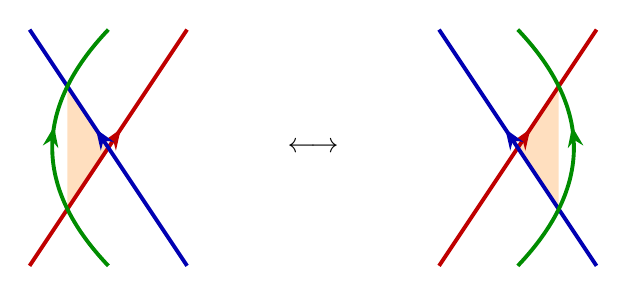
\begin{tikzpicture}[scale=1.0, >=Stealth,
   str/.style={line width=1.4pt, postaction={decorate,
      decoration={markings, mark=at position 0.58 with {\arrow{Stealth[length=2.6mm]}}}}}]
  \begin{scope}[shift={(-2.6,0)}]
    \path[name path=A] (-1,-1.5) -- (1,1.5);
    \path[name path=B] (1,-1.5) -- (-1,1.5);
    \path[name path=C] (0,-1.5) .. controls (-0.95,-0.5) and (-0.95,0.5) .. (0,1.5);
    \path[name intersections={of=A and B, name=iAB}];
    \path[name intersections={of=A and C, name=iAC}];
    \path[name intersections={of=B and C, name=iBC}];
    \fill[orange!25] (iAB-1)--(iAC-1)--(iBC-1)--cycle;
    \draw[str, red!75!black]   (-1,-1.5) -- (1,1.5);
    \draw[str, blue!70!black]  (1,-1.5) -- (-1,1.5);
    \draw[str, green!55!black] (0,-1.5) .. controls (-0.95,-0.5) and (-0.95,0.5) .. (0,1.5);
  \end{scope}
  \node at (0,0) {$\longleftrightarrow$};
  \begin{scope}[shift={(2.6,0)}]
    \path[name path=A2] (-1,-1.5) -- (1,1.5);
    \path[name path=B2] (1,-1.5) -- (-1,1.5);
    \path[name path=C2] (0,-1.5) .. controls (0.95,-0.5) and (0.95,0.5) .. (0,1.5);
    \path[name intersections={of=A2 and B2, name=jAB}];
    \path[name intersections={of=A2 and C2, name=jAC}];
    \path[name intersections={of=B2 and C2, name=jBC}];
    \fill[orange!25] (jAB-1)--(jAC-1)--(jBC-1)--cycle;
    \draw[str, red!75!black]   (-1,-1.5) -- (1,1.5);
    \draw[str, blue!70!black]  (1,-1.5) -- (-1,1.5);
    \draw[str, green!55!black] (0,-1.5) .. controls (0.95,-0.5) and (0.95,0.5) .. (0,1.5);
  \end{scope}
\end{tikzpicture}

\end{document}

%% ====================================================================
%% 보관 영역 (\end{document} 이후) — 컴파일된 코드 누적 보관.
%% 컴파일: 위 \begin{document}...\end{document} 사이에 코드 하나만 두고
%%   cd assets/diagrams/Math/Mirror_Symmetry && latex -shell-escape Mirror_Symmetry.tex
%% 생성된 png를 assets/images/Math/Mirror_Symmetry/{글제목}-n.png 로 이동.
%% ====================================================================

%% 고전 Pieri: (1)에 2 box를 horizontal strip으로 추가 → (3), (2,1) (Quantum_Pieri_Rule-1.png)
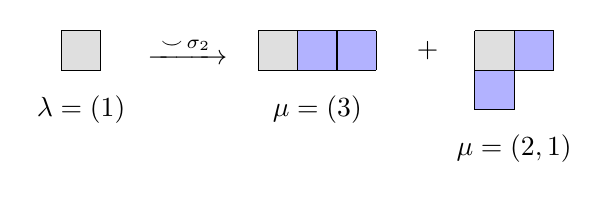
\begin{tikzpicture}[scale=0.5]
  \begin{scope}[shift={(0,0)}]
    \fill[gray!25] (0,0) rectangle (1,1);
    \draw (0,0) grid (1,1);
    \node at (0.5,-1) {$\lambda=(1)$};
  \end{scope}
  \node at (3.2,0.5) {$\xrightarrow{\;\smile\,\sigma_2\;}$};
  \begin{scope}[shift={(5,0)}]
    \fill[gray!25] (0,0) rectangle (1,1);
    \fill[blue!30] (1,0) rectangle (3,1);
    \draw (0,0) grid (3,1);
    \node at (1.5,-1) {$\mu=(3)$};
  \end{scope}
  \node at (9.3,0.5) {$+$};
  \begin{scope}[shift={(10.5,0)}]
    \fill[gray!25] (0,0) rectangle (1,1);
    \fill[blue!30] (1,0) rectangle (2,1);
    \fill[blue!30] (0,-1) rectangle (1,0);
    \draw (0,0) grid (2,1);
    \draw (0,-1) grid (1,1);
    \node at (1,-2) {$\mu=(2,1)$};
  \end{scope}
\end{tikzpicture}

%% rim hook: Gr(2,4)에서 직사각형(2x2) 밖 (3,1)의 4-rim hook 제거 → ∅, +q (Quantum_Pieri_Rule-2.png)
\begin{tikzpicture}[scale=0.5]
  \begin{scope}[shift={(0,0)}]
    \fill[red!20] (0,0) rectangle (3,1);
    \fill[red!20] (0,-1) rectangle (1,0);
    \draw (0,0) grid (3,1);
    \draw (0,-1) grid (1,0);
    \draw[blue, very thick, dashed] (0,-2) rectangle (2,0);
    \node at (1.5,-2.8) {$\mu=(3,1)$};
  \end{scope}
  \node at (5.8,-0.5) {$\xrightarrow{\;4\text{-rim hook}\ \text{제거}\;}$};
  \node at (9.8,-0.5) {$q\,\sigma_\emptyset = q$};
\end{tikzpicture}

%% cohook: box (i,j)의 cohook = 행 왼쪽 + 열 위쪽 (Cluster_Monomial_Basis-1.png)
\begin{tikzpicture}[scale=0.55]
  \draw[gray!50, very thick, dashed] (0,0) rectangle (3,-3);
  \fill[gray!20] (0,0) rectangle (3,-2);
  \draw (0,0) grid (3,-2);
  \fill[blue!25] (0,-1) rectangle (1,-2);
  \fill[orange!30] (1,0) rectangle (2,-1);
  \draw[very thick] (1,-1) rectangle (2,-2);
  \draw (0,0) grid (3,-2);
  \node at (1.5,-1.5) {\scriptsize $(i,j)$};
  \node[blue!60!black] at (0.5,-2.6) {\scriptsize row 왼쪽};
  \node[orange!70!black] at (2.7,0.5) {\scriptsize col 위쪽};
  \node at (1.5,-3.7) {\scriptsize $\lambda=(n\!-\!k)^a$의 cohook};
\end{tikzpicture}

%% Gr(2,4) Gelfand-Tsetlin pattern: interlacing (Newton_Okounkov_Body-1.png)
\begin{tikzpicture}[scale=1.0, >=Stealth]
  \node (a) at (0,0) {$a$};
  \node (b) at (2,0) {$b$};
  \node (c) at (1,-1) {$c$};
  \node (d) at (3,-1) {$d$};
  \node (e) at (2,-2) {$e$};
  \draw[->, gray] (a)--(c); \draw[->, gray] (c)--(b);
  \draw[->, gray] (c)--(e); \draw[->, gray] (e)--(d);
  \draw[->, gray] (b)--(d);
  \node[font=\scriptsize, gray!70!black] at (0.4,-0.55) {$\geq$};
  \node[font=\scriptsize, gray!70!black] at (1.6,-0.55) {$\geq$};
  \node[font=\scriptsize, gray!70!black] at (1.4,-1.55) {$\geq$};
  \node[font=\scriptsize, gray!70!black] at (2.6,-1.55) {$\geq$};
  \node[font=\footnotesize] at (4.8,-1) {$a\geq c\geq b,$};
  \node[font=\footnotesize] at (4.85,-1.55) {$c\geq e\geq d$};
  \node[font=\scriptsize] at (1,-2.8) {$Gr(2,4)$의 GT pattern};
\end{tikzpicture}

%% quiver Q^lambda for lambda=(4,4,2): head-over-tails (Schubert_Variety_Mirror-1.png)
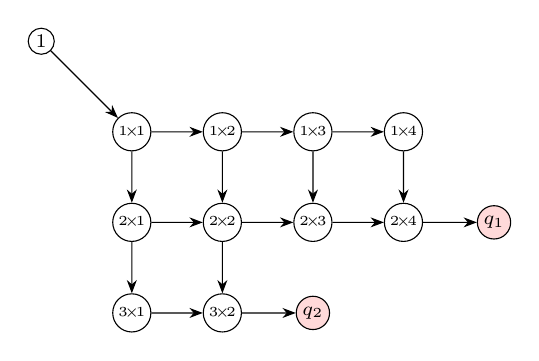
\begin{tikzpicture}[scale=1.15, >=Stealth,
   v/.style={circle, draw, inner sep=1.2pt, font=\scriptsize},
   q/.style={circle, draw, fill=red!15, inner sep=1.2pt, font=\scriptsize}]
  \foreach \i/\jmax in {1/4, 2/4, 3/2}{
    \foreach \j in {1,...,\jmax}{
      \node[v] (n\i\j) at (\j,-\i) {$\scriptstyle \i\!\times\!\j$};
    }
  }
  \node[v] (v0) at (0,0) {$1$};
  \draw[->] (v0) -- (n11);
  \draw[->] (n11)--(n12); \draw[->] (n12)--(n13); \draw[->] (n13)--(n14);
  \draw[->] (n21)--(n22); \draw[->] (n22)--(n23); \draw[->] (n23)--(n24);
  \draw[->] (n31)--(n32);
  \draw[->] (n11)--(n21); \draw[->] (n12)--(n22); \draw[->] (n13)--(n23); \draw[->] (n14)--(n24);
  \draw[->] (n21)--(n31); \draw[->] (n22)--(n32);
  \node[q] (q1) at (5,-2) {$q_1$};
  \node[q] (q2) at (3,-3) {$q_2$};
  \draw[->] (n24) -- (q1);
  \draw[->] (n32) -- (q2);
\end{tikzpicture}

%% 3항 Plücker 관계식: 원 위 S(회색)와 a<b<c<d, 대각선(ac,bd 교차)·변(비교차) (Postnikov_Diagram_and_Plabic_Graph-1.png)
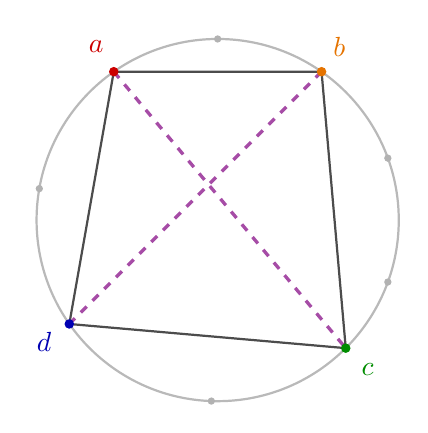
\begin{tikzpicture}[scale=1.15]
  \def\R{2}
  \draw[gray!55, thick] (0,0) circle (\R);
  \coordinate (a) at (125:\R);
  \coordinate (b) at (55:\R);
  \coordinate (c) at (315:\R);
  \coordinate (d) at (215:\R);
  \draw[black!70, thick] (a)--(b)--(c)--(d)--cycle;        % 변 (비교차 현)
  \draw[violet!70, very thick, dashed] (a)--(c);           % 대각선 (교차 현)
  \draw[violet!70, very thick, dashed] (b)--(d);
  \foreach \ang in {90, 20, 340, 268, 170}{                % S에 해당하는 회색 점
    \fill[gray!60] (\ang:\R) circle (1.15pt);
  }
  \fill[red!80!black]    (a) circle (1.5pt);
  \fill[orange!90!black] (b) circle (1.5pt);
  \fill[green!55!black]  (c) circle (1.5pt);
  \fill[blue!70!black]   (d) circle (1.5pt);
  \node[red!80!black]    at (125:{\R+0.34}) {$a$};
  \node[orange!90!black] at (55:{\R+0.34})  {$b$};
  \node[green!55!black]  at (315:{\R+0.34}) {$c$};
  \node[blue!70!black]   at (215:{\R+0.34}) {$d$};
\end{tikzpicture}

%% plabic graph 예시: Gr(1,4) white star, trip permutation i->i+1 (Postnikov_Diagram_and_Plabic_Graph-2.png)
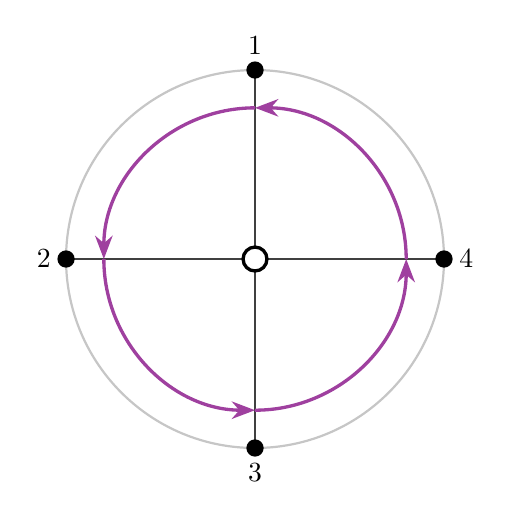
\begin{tikzpicture}[scale=1.2, >=Stealth]
  \def\R{2}
  \draw[gray!45, thick] (0,0) circle (\R);
  \foreach \ang in {90,180,270,0}{ \draw[black!75, thick] (0,0)--(\ang:\R); }
  \draw[fill=white, very thick] (0,0) circle (3.6pt);
  \foreach \ang/\lab/\pos in {90/1/{above}, 180/2/{left}, 270/3/{below}, 0/4/{right}}{
    \fill[black] (\ang:\R) circle (2.6pt);
    \node[\pos=2pt] at (\ang:\R) {$\lab$};
  }
  \foreach \a/\b in {90/180, 180/270, 270/360, 0/90}{
    \draw[violet!75, very thick, ->] (\a:1.6) arc (\a:\b:1.6);
  }
\end{tikzpicture}

%% def5 예시: n=4, 같은 색(white) internal vertex 둘, 점선 boundary (Postnikov_Diagram_and_Plabic_Graph-2.png)
\begin{tikzpicture}[scale=1.3, >=Stealth,
   bv/.style={fill=black, circle, inner sep=1.7pt},
   wv/.style={draw=black, very thick, fill=white, circle, inner sep=3.2pt}]
  \fill[white] (-2.95,-2.95) rectangle (2.95,2.95);
  \def\R{2}
  \draw[gray!60, thick, densely dashed] (0,0) circle (\R);
  \coordinate (W1) at (-0.75,0); \coordinate (W2) at (0.75,0);
  \coordinate (b1) at (135:\R); \coordinate (b2) at (225:\R);
  \coordinate (b3) at (315:\R); \coordinate (b4) at (45:\R);
  \draw[black!80, thick] (W1)--(b1) (W1)--(b2) (W1)--(W2) (W2)--(b3) (W2)--(b4);
  \node[wv] at (W1) {}; \node[wv] at (W2) {};
  \foreach \p/\lab/\pos in {b1/1/{above left}, b2/2/{below left}, b3/3/{below right}, b4/4/{above right}}{
     \node[bv] at (\p) {}; \node[\pos=1pt] at (\p) {$\lab$}; }
\end{tikzpicture}

%% ex7: G(white 2개) --수축--> G'(white 1개), trip 2->3 굵게 (Postnikov_Diagram_and_Plabic_Graph-3.png)
\begin{tikzpicture}[scale=1.0, >=Stealth,
   bv/.style={fill=black, circle, inner sep=1.6pt},
   wv/.style={draw=black, very thick, fill=white, circle, inner sep=3pt},
   trip/.style={violet!75, line width=1.8pt, postaction={decorate,
      decoration={markings, mark=at position #1 with {\arrow{Stealth[length=3mm]}}}}}]
  \fill[white] (-5.6,-2.7) rectangle (5.6,2.7);
  \begin{scope}[shift={(-3,0)}]
    \def\R{1.7}
    \draw[gray!60, thick, densely dashed] (0,0) circle (\R);
    \coordinate (W1) at (-0.62,0); \coordinate (W2) at (0.62,0);
    \coordinate (b1) at (135:\R); \coordinate (b2) at (225:\R);
    \coordinate (b3) at (315:\R); \coordinate (b4) at (45:\R);
    \draw[black!80, thick] (W1)--(b1) (W2)--(b4);
    \draw[trip=0.52] (b2)--(W1)--(W2)--(b3);
    \node[wv] at (W1) {}; \node[wv] at (W2) {};
    \foreach \p/\lab/\pos in {b1/1/{above left}, b2/2/{below left}, b3/3/{below right}, b4/4/{above right}}{
       \node[bv] at (\p) {}; \node[\pos=1pt, font=\small] at (\p) {$\lab$}; }
    \node[font=\small] at (0,-\R-0.55) {$\Gamma$};
  \end{scope}
  \draw[-{Stealth[length=3mm]}, line width=1pt] (-1.0,0)--(1.0,0);
  \node[font=\small] at (0,0.34) {수축};
  \begin{scope}[shift={(3,0)}]
    \def\R{1.7}
    \draw[gray!60, thick, densely dashed] (0,0) circle (\R);
    \coordinate (W) at (0,0);
    \coordinate (b1) at (135:\R); \coordinate (b2) at (225:\R);
    \coordinate (b3) at (315:\R); \coordinate (b4) at (45:\R);
    \draw[black!80, thick] (W)--(b1) (W)--(b4);
    \draw[trip=0.62] (b2)--(W)--(b3);
    \node[wv] at (W) {};
    \foreach \p/\lab/\pos in {b1/1/{above left}, b2/2/{below left}, b3/3/{below right}, b4/4/{above right}}{
       \node[bv] at (\p) {}; \node[\pos=1pt, font=\small] at (\p) {$\lab$}; }
    \node[font=\small] at (0,-\R-0.55) {$\Gamma'$};
  \end{scope}
\end{tikzpicture}

%% def5 예시: n=4, 빈 원 internal vertex 둘, 점선 boundary (invert용) (Postnikov_Diagram_and_Plabic_Graph-2.png)
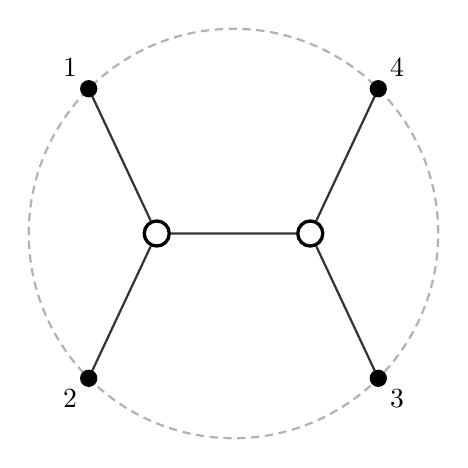
\begin{tikzpicture}[scale=1.3, >=Stealth,
   wv/.style={draw=black, very thick, fill=none, circle, inner sep=3.2pt}]
  \def\R{2}
  \draw[gray!60, thick, densely dashed] (0,0) circle (\R);
  \node[wv] (W1) at (-0.75,0) {};
  \node[wv] (W2) at (0.75,0) {};
  \coordinate (b1) at (135:\R); \coordinate (b2) at (225:\R);
  \coordinate (b3) at (315:\R); \coordinate (b4) at (45:\R);
  \draw[black!80, thick] (W1)--(b1) (W1)--(b2) (W1)--(W2) (W2)--(b3) (W2)--(b4);
  \foreach \p/\lab/\pos in {b1/1/{above left}, b2/2/{below left}, b3/3/{below right}, b4/4/{above right}}{
     \fill[black] (\p) circle (2.4pt); \node[\pos=1pt] at (\p) {$\lab$}; }
\end{tikzpicture}

%% ex7: G(빈 원 2개) --수축--> G'(빈 원 1개), trip 2->3 굵게 (invert용) (Postnikov_Diagram_and_Plabic_Graph-3.png)
\begin{tikzpicture}[scale=1.0, >=Stealth,
   wv/.style={draw=black, very thick, fill=none, circle, inner sep=3pt},
   trip/.style={violet!75, line width=1.8pt, postaction={decorate,
      decoration={markings, mark=at position #1 with {\arrow{Stealth[length=3mm]}}}}}]
  \begin{scope}[shift={(-3,0)}]
    \def\R{1.7}
    \draw[gray!60, thick, densely dashed] (0,0) circle (\R);
    \node[wv] (W1) at (-0.62,0) {}; \node[wv] (W2) at (0.62,0) {};
    \coordinate (b1) at (135:\R); \coordinate (b2) at (225:\R);
    \coordinate (b3) at (315:\R); \coordinate (b4) at (45:\R);
    \draw[black!80, thick] (W1)--(b1) (W2)--(b4);
    \draw[trip=0.52] (b2)--(W1)--(W2)--(b3);
    \foreach \p/\lab/\pos in {b1/1/{above left}, b2/2/{below left}, b3/3/{below right}, b4/4/{above right}}{
       \fill[black] (\p) circle (1.7pt); \node[\pos=1pt, font=\small] at (\p) {$\lab$}; }
    \node[font=\small] at (0,-\R-0.55) {$\Gamma$};
  \end{scope}
  \draw[-{Stealth[length=3mm]}, line width=1pt] (-1.0,0)--(1.0,0);
  \node[font=\small] at (0,0.34) {수축};
  \begin{scope}[shift={(3,0)}]
    \def\R{1.7}
    \draw[gray!60, thick, densely dashed] (0,0) circle (\R);
    \node[wv] (W) at (0,0) {};
    \coordinate (b1) at (135:\R); \coordinate (b2) at (225:\R);
    \coordinate (b3) at (315:\R); \coordinate (b4) at (45:\R);
    \draw[black!80, thick] (W)--(b1) (W)--(b4);
    \draw[trip=0.62] (b2)--(W)--(b3);
    \foreach \p/\lab/\pos in {b1/1/{above left}, b2/2/{below left}, b3/3/{below right}, b4/4/{above right}}{
       \fill[black] (\p) circle (1.7pt); \node[\pos=1pt, font=\small] at (\p) {$\lab$}; }
    \node[font=\small] at (0,-\R-0.55) {$\Gamma'$};
  \end{scope}
\end{tikzpicture}

%% ex7: Γ (빈 원 2개), trip 2->3 굵게 (Postnikov_Diagram_and_Plabic_Graph-3.png)
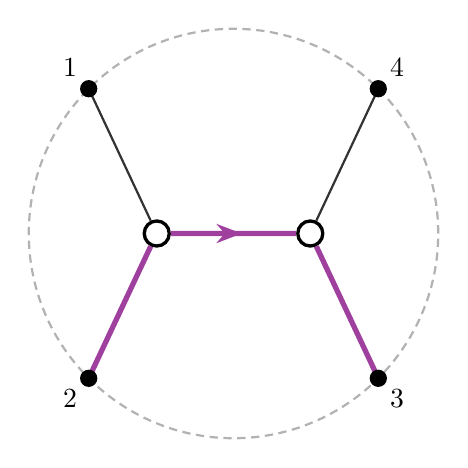
\begin{tikzpicture}[scale=1.3, >=Stealth,
   wv/.style={draw=black, very thick, fill=none, circle, inner sep=3.2pt},
   trip/.style={violet!75, line width=1.9pt, postaction={decorate,
      decoration={markings, mark=at position #1 with {\arrow{Stealth[length=3.2mm]}}}}}]
  \def\R{2}
  \draw[gray!60, thick, densely dashed] (0,0) circle (\R);
  \node[wv] (W1) at (-0.75,0) {}; \node[wv] (W2) at (0.75,0) {};
  \coordinate (b1) at (135:\R); \coordinate (b2) at (225:\R);
  \coordinate (b3) at (315:\R); \coordinate (b4) at (45:\R);
  \draw[black!80, thick] (W1)--(b1) (W2)--(b4);
  \draw[trip=0.52] (b2)--(W1)--(W2)--(b3);
  \foreach \p/\lab/\pos in {b1/1/{above left}, b2/2/{below left}, b3/3/{below right}, b4/4/{above right}}{
     \fill[black] (\p) circle (2.4pt); \node[\pos=1pt] at (\p) {$\lab$}; }
\end{tikzpicture}

%% ex7: Γ' (빈 원 1개, 수축 결과), trip 2->3 굵게 (Postnikov_Diagram_and_Plabic_Graph-4.png)
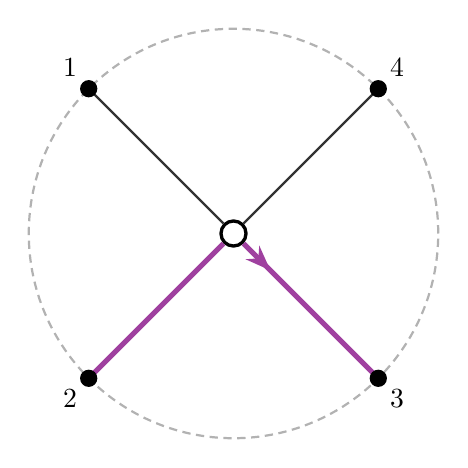
\begin{tikzpicture}[scale=1.3, >=Stealth,
   wv/.style={draw=black, very thick, fill=none, circle, inner sep=3.2pt},
   trip/.style={violet!75, line width=1.9pt, postaction={decorate,
      decoration={markings, mark=at position #1 with {\arrow{Stealth[length=3.2mm]}}}}}]
  \def\R{2}
  \draw[gray!60, thick, densely dashed] (0,0) circle (\R);
  \node[wv] (W) at (0,0) {};
  \coordinate (b1) at (135:\R); \coordinate (b2) at (225:\R);
  \coordinate (b3) at (315:\R); \coordinate (b4) at (45:\R);
  \draw[black!80, thick] (W)--(b1) (W)--(b4);
  \draw[trip=0.6] (b2)--(W)--(b3);
  \foreach \p/\lab/\pos in {b1/1/{above left}, b2/2/{below left}, b3/3/{below right}, b4/4/{above right}}{
     \fill[black] (\p) circle (2.4pt); \node[\pos=1pt] at (\p) {$\lab$}; }
\end{tikzpicture}

%% def10: Gr(2,4) Postnikov diagram, 4 strands i->i+2 (Postnikov_Diagram_and_Plabic_Graph-5.png)
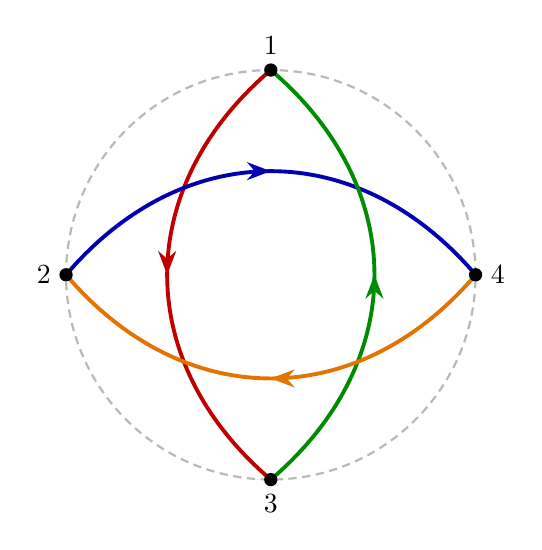
\begin{tikzpicture}[scale=1.3, >=Stealth,
   bdot/.style={fill=black, circle, inner sep=1.7pt},
   strand/.style={line width=1.4pt, postaction={decorate,
      decoration={markings, mark=at position 0.5 with {\arrow{Stealth[length=3mm]}}}}}]
  \def\R{2}
  \draw[gray!55, thick, densely dashed] (0,0) circle (\R);
  \coordinate (b1) at (90:\R); \coordinate (b2) at (180:\R);
  \coordinate (b3) at (270:\R); \coordinate (b4) at (0:\R);
  \draw[strand, red!75!black]    (b1) .. controls (-1.35,0.85) and (-1.35,-0.85) .. (b3);
  \draw[strand, blue!70!black]   (b2) .. controls (-0.85,1.35) and (0.85,1.35) .. (b4);
  \draw[strand, green!55!black]  (b3) .. controls (1.35,-0.85) and (1.35,0.85) .. (b1);
  \draw[strand, orange!90!black] (b4) .. controls (0.85,-1.35) and (-0.85,-1.35) .. (b2);
  \foreach \p/\lab/\pos in {b1/1/{above}, b2/2/{left}, b3/3/{below}, b4/4/{right}}{
     \node[bdot] at (\p) {}; \node[\pos=2pt] at (\p) {$\lab$}; }
\end{tikzpicture}

%% prop11: Gr(2,4) plabic graph(square), face label 없는 plain 버전 (Postnikov_Diagram_and_Plabic_Graph-6.png)
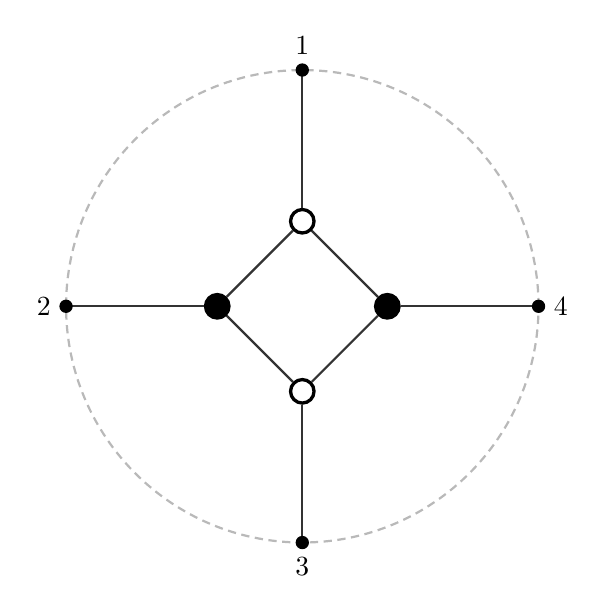
\begin{tikzpicture}[scale=1.5, >=Stealth,
   bdot/.style={fill=black, circle, inner sep=1.7pt},
   wv/.style={draw=black, very thick, fill=none, circle, inner sep=3pt},
   bv/.style={draw=black, very thick, fill=black, circle, inner sep=3pt}]
  \def\R{2}
  \draw[gray!55, thick, densely dashed] (0,0) circle (\R);
  \node[wv] (N) at (0,0.72) {}; \node[bv] (E) at (0.72,0) {};
  \node[wv] (S) at (0,-0.72) {}; \node[bv] (W) at (-0.72,0) {};
  \coordinate (b1) at (90:\R); \coordinate (b2) at (180:\R);
  \coordinate (b3) at (270:\R); \coordinate (b4) at (0:\R);
  \draw[black!80, thick] (N)--(E)--(S)--(W)--(N);
  \draw[black!80, thick] (N)--(b1) (W)--(b2) (S)--(b3) (E)--(b4);
  \foreach \p/\lab/\pos in {b1/1/{above}, b2/2/{left}, b3/3/{below}, b4/4/{right}}{
     \node[bdot] at (\p) {}; \node[\pos=2pt] at (\p) {$\lab$}; }
\end{tikzpicture}

%% def12: Gr(2,4) plabic graph(square) + face labels (Postnikov_Diagram_and_Plabic_Graph-7.png)
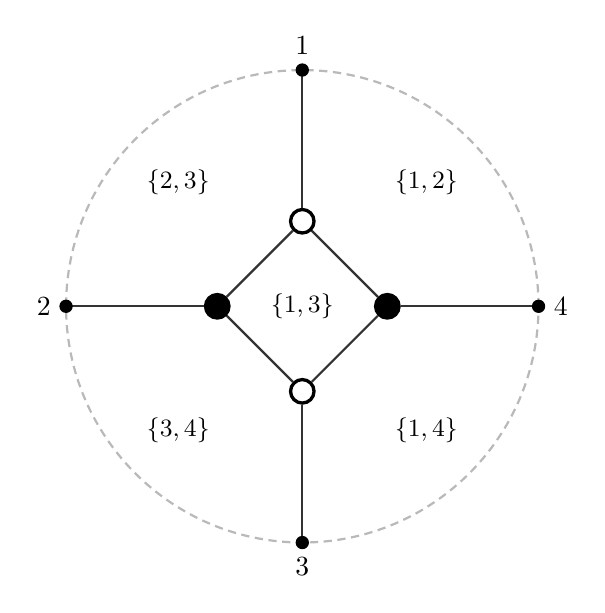
\begin{tikzpicture}[scale=1.5, >=Stealth,
   bdot/.style={fill=black, circle, inner sep=1.7pt},
   wv/.style={draw=black, very thick, fill=none, circle, inner sep=3pt},
   bv/.style={draw=black, very thick, fill=black, circle, inner sep=3pt}]
  \def\R{2}
  \draw[gray!55, thick, densely dashed] (0,0) circle (\R);
  \node[wv] (N) at (0,0.72) {}; \node[bv] (E) at (0.72,0) {};
  \node[wv] (S) at (0,-0.72) {}; \node[bv] (W) at (-0.72,0) {};
  \coordinate (b1) at (90:\R); \coordinate (b2) at (180:\R);
  \coordinate (b3) at (270:\R); \coordinate (b4) at (0:\R);
  \draw[black!80, thick] (N)--(E)--(S)--(W)--(N);
  \draw[black!80, thick] (N)--(b1) (W)--(b2) (S)--(b3) (E)--(b4);
  \foreach \p/\lab/\pos in {b1/1/{above}, b2/2/{left}, b3/3/{below}, b4/4/{right}}{
     \node[bdot] at (\p) {}; \node[\pos=2pt] at (\p) {$\lab$}; }
  \node[font=\small] at (0,0) {$\{1,3\}$};
  \node[font=\small] at (1.05,1.05) {$\{1,2\}$};
  \node[font=\small] at (-1.05,1.05) {$\{2,3\}$};
  \node[font=\small] at (-1.05,-1.05) {$\{3,4\}$};
  \node[font=\small] at (1.05,-1.05) {$\{1,4\}$};
\end{tikzpicture}

%% def10: Gr(2,4) Postnikov diagram, 4 strands i->i+2, over/under alternating (Postnikov_Diagram_and_Plabic_Graph-5.png)
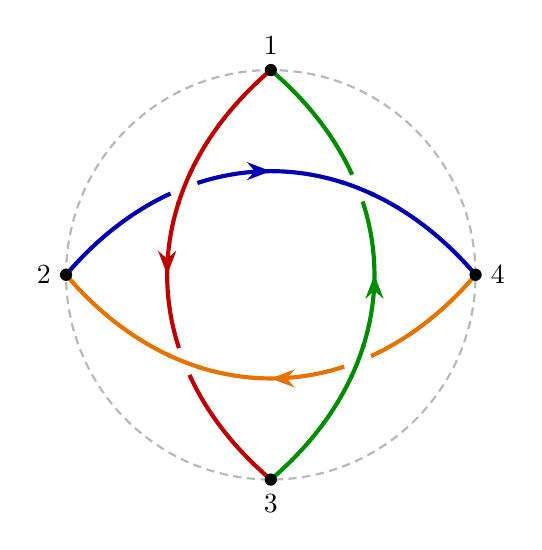
\begin{tikzpicture}[scale=1.3, >=Stealth,
   strand/.style={line width=1.5pt, postaction={decorate,
      decoration={markings, mark=at position 0.5 with {\arrow{Stealth[length=3mm]}}}}},
   bare/.style={line width=1.5pt}]
  \def\R{2}
  \draw[gray!55, thick, densely dashed] (0,0) circle (\R);
  \coordinate (b1) at (90:\R); \coordinate (b2) at (180:\R);
  \coordinate (b3) at (270:\R); \coordinate (b4) at (0:\R);
  \draw[strand, red!75!black,    name path=sR] (b1) .. controls (-1.35,0.85) and (-1.35,-0.85) .. (b3);
  \draw[strand, blue!70!black,   name path=sB] (b2) .. controls (-0.85,1.35) and (0.85,1.35) .. (b4);
  \draw[strand, green!55!black,  name path=sG] (b3) .. controls (1.35,-0.85) and (1.35,0.85) .. (b1);
  \draw[strand, orange!90!black, name path=sO] (b4) .. controls (0.85,-1.35) and (-0.85,-1.35) .. (b2);
  \path[name intersections={of=sR and sB, name=cNW}];
  \path[name intersections={of=sB and sG, name=cNE}];
  \path[name intersections={of=sG and sO, name=cSE}];
  \path[name intersections={of=sO and sR, name=cSW}];
  % over: NW red, NE blue, SE green, SW orange
  \fill[white] (cNW-1) circle (4pt);
  \begin{scope}\clip (cNW-1) circle (5pt);\draw[bare, red!75!black] (b1) .. controls (-1.35,0.85) and (-1.35,-0.85) .. (b3);\end{scope}
  \fill[white] (cNE-1) circle (4pt);
  \begin{scope}\clip (cNE-1) circle (5pt);\draw[bare, blue!70!black] (b2) .. controls (-0.85,1.35) and (0.85,1.35) .. (b4);\end{scope}
  \fill[white] (cSE-1) circle (4pt);
  \begin{scope}\clip (cSE-1) circle (5pt);\draw[bare, green!55!black] (b3) .. controls (1.35,-0.85) and (1.35,0.85) .. (b1);\end{scope}
  \fill[white] (cSW-1) circle (4pt);
  \begin{scope}\clip (cSW-1) circle (5pt);\draw[bare, orange!90!black] (b4) .. controls (0.85,-1.35) and (-0.85,-1.35) .. (b2);\end{scope}
  \foreach \p/\lab/\pos in {b1/1/{above}, b2/2/{left}, b3/3/{below}, b4/4/{right}}{
     \fill[black] (\p) circle (1.7pt); \node[\pos=2pt] at (\p) {$\lab$}; }
\end{tikzpicture}

%% def10: Gr(2,4) Postnikov diagram, i->i+2, over/under via transparent gaps (Postnikov_Diagram_and_Plabic_Graph-5.png)
\begin{tikzpicture}[scale=1.3, >=Stealth,
   strand/.style={line width=1.5pt, postaction={decorate,
      decoration={markings, mark=at position 0.5 with {\arrow{Stealth[length=3mm]}}}}}]
  \def\R{2}
  \draw[gray!55, thick, densely dashed] (0,0) circle (\R);
  \coordinate (b1) at (90:\R); \coordinate (b2) at (180:\R);
  \coordinate (b3) at (270:\R); \coordinate (b4) at (0:\R);
  \path[name path=sR] (b1) .. controls (-1.35,0.85) and (-1.35,-0.85) .. (b3);
  \path[name path=sB] (b2) .. controls (-0.85,1.35) and (0.85,1.35) .. (b4);
  \path[name path=sG] (b3) .. controls (1.35,-0.85) and (1.35,0.85) .. (b1);
  \path[name path=sO] (b4) .. controls (0.85,-1.35) and (-0.85,-1.35) .. (b2);
  \path[name intersections={of=sR and sB, name=cNW}];
  \path[name intersections={of=sB and sG, name=cNE}];
  \path[name intersections={of=sG and sO, name=cSE}];
  \path[name intersections={of=sO and sR, name=cSW}];
  % each strand: transparent gap at its UNDER crossing (red@SW, blue@NW, green@NE, orange@SE)
  \begin{scope}\clip[even odd rule] (-2.7,-2.7) rectangle (2.7,2.7) (cSW-1) circle (4pt);
    \draw[strand, red!75!black] (b1) .. controls (-1.35,0.85) and (-1.35,-0.85) .. (b3);\end{scope}
  \begin{scope}\clip[even odd rule] (-2.7,-2.7) rectangle (2.7,2.7) (cNW-1) circle (4pt);
    \draw[strand, blue!70!black] (b2) .. controls (-0.85,1.35) and (0.85,1.35) .. (b4);\end{scope}
  \begin{scope}\clip[even odd rule] (-2.7,-2.7) rectangle (2.7,2.7) (cNE-1) circle (4pt);
    \draw[strand, green!55!black] (b3) .. controls (1.35,-0.85) and (1.35,0.85) .. (b1);\end{scope}
  \begin{scope}\clip[even odd rule] (-2.7,-2.7) rectangle (2.7,2.7) (cSE-1) circle (4pt);
    \draw[strand, orange!90!black] (b4) .. controls (0.85,-1.35) and (-0.85,-1.35) .. (b2);\end{scope}
  \foreach \p/\lab/\pos in {b1/1/{above}, b2/2/{left}, b3/3/{below}, b4/4/{right}}{
     \fill[black] (\p) circle (1.7pt); \node[\pos=2pt] at (\p) {$\lab$}; }
\end{tikzpicture}

%% def10: Gr(2,4) Postnikov diagram, i->i+2, over/under via transparent gaps (Postnikov_Diagram_and_Plabic_Graph-5.png)
\begin{tikzpicture}[scale=1.3, >=Stealth, every path/.append style={line width=1.5pt}]
  \def\R{2}
  \draw[gray!55, thick, densely dashed] (0,0) circle (\R);
  \coordinate (b1) at (90:\R); \coordinate (b2) at (180:\R);
  \coordinate (b3) at (270:\R); \coordinate (b4) at (0:\R);
  \path[name path=sR] (b1) .. controls (-1.35,0.85) and (-1.35,-0.85) .. (b3);
  \path[name path=sB] (b2) .. controls (-0.85,1.35) and (0.85,1.35) .. (b4);
  \path[name path=sG] (b3) .. controls (1.35,-0.85) and (1.35,0.85) .. (b1);
  \path[name path=sO] (b4) .. controls (0.85,-1.35) and (-0.85,-1.35) .. (b2);
  \path[name intersections={of=sR and sB, name=cNW}];
  \path[name intersections={of=sB and sG, name=cNE}];
  \path[name intersections={of=sG and sO, name=cSE}];
  \path[name intersections={of=sO and sR, name=cSW}];
  \begin{scope}\clip[even odd rule] (-2.7,-2.7) rectangle (2.7,2.7) (cSW-1) circle (4pt);
    \draw[red!75!black] (b1) .. controls (-1.35,0.85) and (-1.35,-0.85) .. (b3);\end{scope}
  \begin{scope}\clip[even odd rule] (-2.7,-2.7) rectangle (2.7,2.7) (cNW-1) circle (4pt);
    \draw[blue!70!black] (b2) .. controls (-0.85,1.35) and (0.85,1.35) .. (b4);\end{scope}
  \begin{scope}\clip[even odd rule] (-2.7,-2.7) rectangle (2.7,2.7) (cNE-1) circle (4pt);
    \draw[green!55!black] (b3) .. controls (1.35,-0.85) and (1.35,0.85) .. (b1);\end{scope}
  \begin{scope}\clip[even odd rule] (-2.7,-2.7) rectangle (2.7,2.7) (cSE-1) circle (4pt);
    \draw[orange!90!black] (b4) .. controls (0.85,-1.35) and (-0.85,-1.35) .. (b2);\end{scope}
  % direction arrows at bulges (unclipped, away from crossings)
  \draw[red!75!black,-{Stealth[length=3mm]}]    (-1.012,0.22)--(-1.012,-0.22);
  \draw[blue!70!black,-{Stealth[length=3mm]}]   (-0.22,1.012)--(0.22,1.012);
  \draw[green!55!black,-{Stealth[length=3mm]}]  (1.012,-0.22)--(1.012,0.22);
  \draw[orange!90!black,-{Stealth[length=3mm]}] (0.22,-1.012)--(-0.22,-1.012);
  \foreach \p/\lab/\pos in {b1/1/{above}, b2/2/{left}, b3/3/{below}, b4/4/{right}}{
     \fill[black] (\p) circle (1.7pt); \node[\pos=2pt] at (\p) {$\lab$}; }
\end{tikzpicture}

%% def10: Gr(2,4) Postnikov diagram, i->i+2, over/under via transparent gaps (Postnikov_Diagram_and_Plabic_Graph-5.png)
\begin{tikzpicture}[scale=1.3, >=Stealth, every path/.append style={line width=1.5pt}]
  \def\R{2}
  \draw[gray!55, thick, densely dashed] (0,0) circle (\R);
  \coordinate (b1) at (90:\R); \coordinate (b2) at (180:\R);
  \coordinate (b3) at (270:\R); \coordinate (b4) at (0:\R);
  \path[name path=sR] (b1) .. controls (-1.35,0.85) and (-1.35,-0.85) .. (b3);
  \path[name path=sB] (b2) .. controls (-0.85,1.35) and (0.85,1.35) .. (b4);
  \path[name path=sG] (b3) .. controls (1.35,-0.85) and (1.35,0.85) .. (b1);
  \path[name path=sO] (b4) .. controls (0.85,-1.35) and (-0.85,-1.35) .. (b2);
  \path[name intersections={of=sR and sB, name=cNW}];
  \path[name intersections={of=sB and sG, name=cNE}];
  \path[name intersections={of=sG and sO, name=cSE}];
  \path[name intersections={of=sO and sR, name=cSW}];
  \begin{scope}\path[clip, even odd rule] (-2.7,-2.7) rectangle (2.7,2.7) (cSW-1) circle (4pt);
    \draw[red!75!black] (b1) .. controls (-1.35,0.85) and (-1.35,-0.85) .. (b3);\end{scope}
  \begin{scope}\path[clip, even odd rule] (-2.7,-2.7) rectangle (2.7,2.7) (cNW-1) circle (4pt);
    \draw[blue!70!black] (b2) .. controls (-0.85,1.35) and (0.85,1.35) .. (b4);\end{scope}
  \begin{scope}\path[clip, even odd rule] (-2.7,-2.7) rectangle (2.7,2.7) (cNE-1) circle (4pt);
    \draw[green!55!black] (b3) .. controls (1.35,-0.85) and (1.35,0.85) .. (b1);\end{scope}
  \begin{scope}\path[clip, even odd rule] (-2.7,-2.7) rectangle (2.7,2.7) (cSE-1) circle (4pt);
    \draw[orange!90!black] (b4) .. controls (0.85,-1.35) and (-0.85,-1.35) .. (b2);\end{scope}
  \draw[red!75!black,-{Stealth[length=3mm]}]    (-1.012,0.22)--(-1.012,-0.22);
  \draw[blue!70!black,-{Stealth[length=3mm]}]   (-0.22,1.012)--(0.22,1.012);
  \draw[green!55!black,-{Stealth[length=3mm]}]  (1.012,-0.22)--(1.012,0.22);
  \draw[orange!90!black,-{Stealth[length=3mm]}] (0.22,-1.012)--(-0.22,-1.012);
  \foreach \p/\lab/\pos in {b1/1/{above}, b2/2/{left}, b3/3/{below}, b4/4/{right}}{
     \fill[black] (\p) circle (1.7pt); \node[\pos=2pt] at (\p) {$\lab$}; }
\end{tikzpicture}

%% def10: Gr(2,4) Postnikov diagram, i->i+2, over/under via transparent gaps (Postnikov_Diagram_and_Plabic_Graph-5.png)
\begin{tikzpicture}[scale=1.3, >=Stealth, every path/.append style={line width=1.5pt}]
  \def\R{2}
  \draw[gray!55, thick, densely dashed] (0,0) circle (\R);
  \coordinate (b1) at (90:\R); \coordinate (b2) at (180:\R);
  \coordinate (b3) at (270:\R); \coordinate (b4) at (0:\R);
  \path[name path=sR] (b1) .. controls (-1.35,0.85) and (-1.35,-0.85) .. (b3);
  \path[name path=sB] (b2) .. controls (-0.85,1.35) and (0.85,1.35) .. (b4);
  \path[name path=sG] (b3) .. controls (1.35,-0.85) and (1.35,0.85) .. (b1);
  \path[name path=sO] (b4) .. controls (0.85,-1.35) and (-0.85,-1.35) .. (b2);
  \path[name intersections={of=sR and sB, name=cNW}];
  \path[name intersections={of=sB and sG, name=cNE}];
  \path[name intersections={of=sG and sO, name=cSE}];
  \path[name intersections={of=sO and sR, name=cSW}];
  \begin{scope}[even odd rule]\clip (-2.7,-2.7) rectangle (2.7,2.7) (cSW-1) circle (4pt);
    \draw[red!75!black] (b1) .. controls (-1.35,0.85) and (-1.35,-0.85) .. (b3);\end{scope}
  \begin{scope}[even odd rule]\clip (-2.7,-2.7) rectangle (2.7,2.7) (cNW-1) circle (4pt);
    \draw[blue!70!black] (b2) .. controls (-0.85,1.35) and (0.85,1.35) .. (b4);\end{scope}
  \begin{scope}[even odd rule]\clip (-2.7,-2.7) rectangle (2.7,2.7) (cNE-1) circle (4pt);
    \draw[green!55!black] (b3) .. controls (1.35,-0.85) and (1.35,0.85) .. (b1);\end{scope}
  \begin{scope}[even odd rule]\clip (-2.7,-2.7) rectangle (2.7,2.7) (cSE-1) circle (4pt);
    \draw[orange!90!black] (b4) .. controls (0.85,-1.35) and (-0.85,-1.35) .. (b2);\end{scope}
  \draw[red!75!black,-{Stealth[length=3mm]}]    (-1.012,0.22)--(-1.012,-0.22);
  \draw[blue!70!black,-{Stealth[length=3mm]}]   (-0.22,1.012)--(0.22,1.012);
  \draw[green!55!black,-{Stealth[length=3mm]}]  (1.012,-0.22)--(1.012,0.22);
  \draw[orange!90!black,-{Stealth[length=3mm]}] (0.22,-1.012)--(-0.22,-1.012);
  \foreach \p/\lab/\pos in {b1/1/{above}, b2/2/{left}, b3/3/{below}, b4/4/{right}}{
     \fill[black] (\p) circle (1.7pt); \node[\pos=2pt] at (\p) {$\lab$}; }
\end{tikzpicture}

%% def10 (CURRENT): Gr(2,4) Postnikov diagram, i->i+2, plain transversal crossings (over/under 제거) (Postnikov_Diagram_and_Plabic_Graph-5.png)
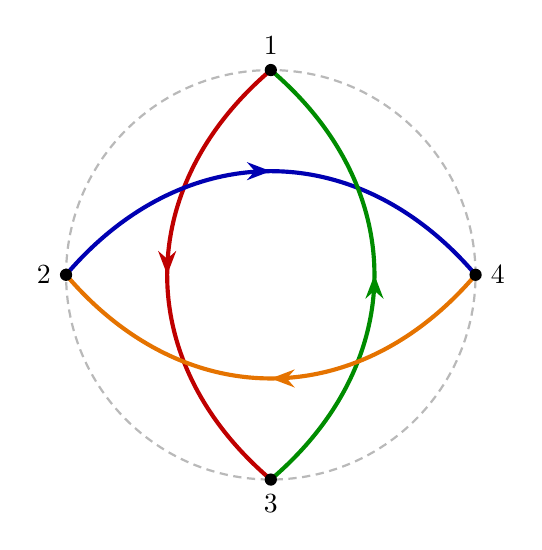
\begin{tikzpicture}[scale=1.3, >=Stealth,
   strand/.style={line width=1.5pt, postaction={decorate,
      decoration={markings, mark=at position 0.5 with {\arrow{Stealth[length=3mm]}}}}}]
  \def\R{2}
  \draw[gray!55, thick, densely dashed] (0,0) circle (\R);
  \coordinate (b1) at (90:\R); \coordinate (b2) at (180:\R);
  \coordinate (b3) at (270:\R); \coordinate (b4) at (0:\R);
  \draw[strand, red!75!black]    (b1) .. controls (-1.35,0.85) and (-1.35,-0.85) .. (b3);
  \draw[strand, blue!70!black]   (b2) .. controls (-0.85,1.35) and (0.85,1.35) .. (b4);
  \draw[strand, green!55!black]  (b3) .. controls (1.35,-0.85) and (1.35,0.85) .. (b1);
  \draw[strand, orange!90!black] (b4) .. controls (0.85,-1.35) and (-0.85,-1.35) .. (b2);
  \foreach \p/\lab/\pos in {b1/1/{above}, b2/2/{left}, b3/3/{below}, b4/4/{right}}{
     \fill[black] (\p) circle (1.7pt); \node[\pos=2pt] at (\p) {$\lab$}; }
\end{tikzpicture}

%% def10 (구버전, 폐기): Gr(2,4) Postnikov diagram, i->i+2, over/under (white gaps -> post-process transparent) (Postnikov_Diagram_and_Plabic_Graph-5.png)
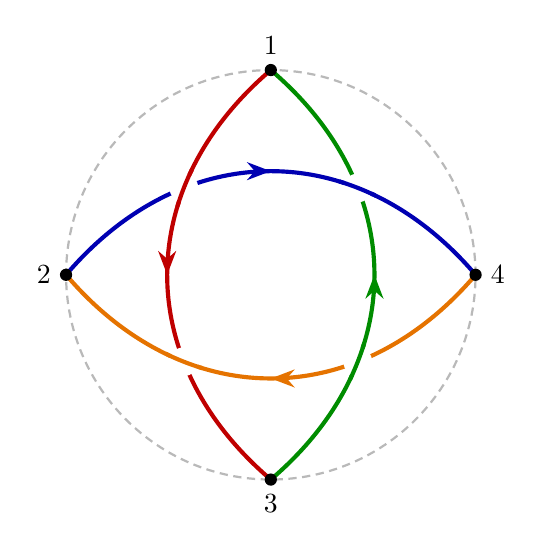
\begin{tikzpicture}[scale=1.3, >=Stealth,
   strand/.style={line width=1.5pt, postaction={decorate,
      decoration={markings, mark=at position 0.5 with {\arrow{Stealth[length=3mm]}}}}},
   bare/.style={line width=1.5pt}]
  \def\R{2}
  \draw[gray!55, thick, densely dashed] (0,0) circle (\R);
  \coordinate (b1) at (90:\R); \coordinate (b2) at (180:\R);
  \coordinate (b3) at (270:\R); \coordinate (b4) at (0:\R);
  \draw[strand, red!75!black,    name path=sR] (b1) .. controls (-1.35,0.85) and (-1.35,-0.85) .. (b3);
  \draw[strand, blue!70!black,   name path=sB] (b2) .. controls (-0.85,1.35) and (0.85,1.35) .. (b4);
  \draw[strand, green!55!black,  name path=sG] (b3) .. controls (1.35,-0.85) and (1.35,0.85) .. (b1);
  \draw[strand, orange!90!black, name path=sO] (b4) .. controls (0.85,-1.35) and (-0.85,-1.35) .. (b2);
  \path[name intersections={of=sR and sB, name=cNW}];
  \path[name intersections={of=sB and sG, name=cNE}];
  \path[name intersections={of=sG and sO, name=cSE}];
  \path[name intersections={of=sO and sR, name=cSW}];
  \fill[white] (cNW-1) circle (4pt);
  \begin{scope}\clip (cNW-1) circle (5.5pt);\draw[bare, red!75!black] (b1) .. controls (-1.35,0.85) and (-1.35,-0.85) .. (b3);\end{scope}
  \fill[white] (cNE-1) circle (4pt);
  \begin{scope}\clip (cNE-1) circle (5.5pt);\draw[bare, blue!70!black] (b2) .. controls (-0.85,1.35) and (0.85,1.35) .. (b4);\end{scope}
  \fill[white] (cSE-1) circle (4pt);
  \begin{scope}\clip (cSE-1) circle (5.5pt);\draw[bare, green!55!black] (b3) .. controls (1.35,-0.85) and (1.35,0.85) .. (b1);\end{scope}
  \fill[white] (cSW-1) circle (4pt);
  \begin{scope}\clip (cSW-1) circle (5.5pt);\draw[bare, orange!90!black] (b4) .. controls (0.85,-1.35) and (-0.85,-1.35) .. (b2);\end{scope}
  \foreach \p/\lab/\pos in {b1/1/{above}, b2/2/{left}, b3/3/{below}, b4/4/{right}}{
     \fill[black] (\p) circle (1.7pt); \node[\pos=2pt] at (\p) {$\lab$}; }
\end{tikzpicture}
